\chapter{OpenGL}

\section{GLSL}

\subsection{screen space derivative}
屏幕空间偏导数
GPU always evaluate fragment/pixel shaders on 2x2 blocks of pixels at a time.

use this techniques for rendering antialiased lines

\begin{figure}[h]
    \centering
    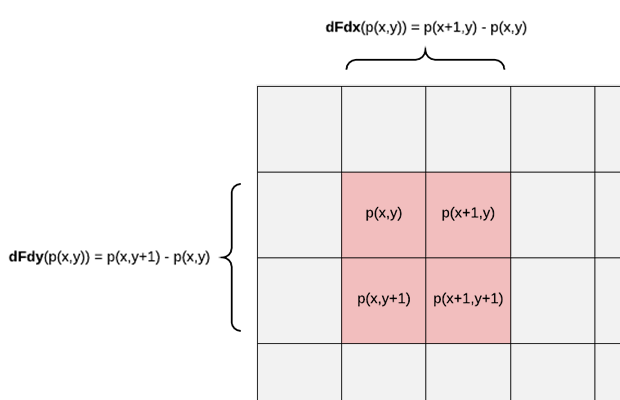
\includegraphics[width=\textwidth]{images/Shader-Derivatives.png}
\end{figure}

antialiasing,AA抗锯齿,对于一张纹理,给定UV坐标后,不仅仅是直接采样,还要考虑周围方形
区域内采样的结果,这个区域就是ddx和ddy给定的区域,在shader中调用texture时,后台进行了处理,
在一些高级的profiles中,还是允许自定义滤波窗口大小的

mipmap,在屏幕空间中,纹理坐标变换剧烈,Derivatives are used during texture sampling to
select the best mipmap level.

\paragraph{fwidth}
GLSL中,fwidth函数返回的是X和Y方向偏导数的绝对值的和,而单方向的偏导数可以通过ddx和ddy获得

注意,这些函数与像素有关,只能在fragment/pixel shader中使用

\section{Coordinate}

OpenGL是右手系坐标

\subsection{Ordinary Coordinate}
普通坐标,

\subsection{Homogeneous Coordinate}
齐次坐标系,为了计算的一致性,使用矩阵可以方便表示旋转,缩放,但是平移就不行了。进行升维操作,
可以把2维扩展维3三维,三维扩展为四维,这样就能保证旋转,缩放,平移都以矩阵形式来表示。

齐次坐标系是计算机图形学的基础,能够明确区分向量和点,同时也易于进行仿射(线性)几何变换。

\subsection{Coordinate Space}
坐标空间是一个相对概念,

\paragraph{Modle Space}
物体空间坐标,局部空间。把物体从局部空间放到世界空间中,需要一个Model Matrix的变换过程。

\paragraph{World Space}
世界空间,就是整个场景的参考坐标系。把场景放到摄像机空间需要一个View Matrix的变换过程。

\paragraph{Eye-Camera Space}
摄像机空间,观察者所在坐标空间中。从观察空间到裁剪空间需要一个Projection Maxtrix的变换过程。

\paragraph{Clip Space}
裁剪空间,
会进行Perspective division透视除法,为了透视效果。

\paragraph{NDC Space}
视口空间, Normalized Device Coordinate Space, 这里与设备进行规范化转换。
需要一个Viewport Matrix转换到屏幕空间中。

OpenGL的坐标原点是左下角,Vulkan的坐标原点是左上角。在共享shader时,就需要注意两种的区别了。


\paragraph{Screen Space}
屏幕空间

\section{Technique Artist}
技术美术

\section{3D Render Library}

\subsection{Render Engine}

\textbf{OpenSceneGraph}

\textbf{bgfx}

\textbf{Armory Engine}\cite{Armory}, Armory is an open-source 3D engine focused on portability, minimal footprint and performance. The renderer is fully scriptable with deferred and forward paths supported out of the box.Written in C, Haxe and WebAssembly, structured as a data-driven engine.

\textbf{UPBGE}\cite{upbge}, is an open-source 3D game engine forked from old Blender Game Engine, deployed with Blender itself. This unified workflow is its main strength as you can make your game from start to end without leave UPBGE.

\textbf{three.js}

\textbf{Babylon.js}


\chapter{Vulkan}

vulkan是控制GPU设备的API,是OpenGL下一代且更底层的API,由OpenGL驱动提供的功能都需要自己实现,包括,同步,进度,内存管理等。
所以vulkan是适合大型复杂的图形渲染,定制性要求很高,OpenGL提供不了的功能。

既然是API,它相比OpenGL的状态机,更符合面向对象设计,与DirectX类似,是C语言的接口,这算是OpenGL切换到Vulkan最直接的感受。

\section{Host-Device}
Vulkan延续OpenGL的Host-Device设计模型,将CPU与GPU看成是一个异步执行的过程,这样CPU可以多线程提供数据给GPU使用。
这也是Vulkan是基于现代GPU渲染模型的一个抽象包装,相比CPU的多缓存与串行执行模型,GPU是高并发和高延迟。

驱动层等于是在系统内存System Memory和GPU的显卡内存Device Memory上,维护了一块内存来保持一致,
对CPU来说就是VkBuffer数据源,对GPU来说就是VkDeviceMemory,

\subsection{Resource}

vulkan的操作基于数据,所有data都存储在resources中,它们被后台内存管理着,构建这些资源大致有两步
\begin{itemize}
    \item {resource is created, ex, vkCreateBuffer}
    \item {resource needs to be backed by memory, 允许应用程序管理内存}
\end{itemize}

\paragraph{buffers}

线性存储块,可拥有存储任何的数据,它同样可以存储图像数据

\paragraph{images}

图像,具有结构性,类型,格式的固定数据


\section{Pipeline}
OpenGL的所有状态都由OpenGL的VM进行管理,而Vulkan相反,把所有渲染状态都放在一个VkPipeline对象上。
包含了所有可编程programable渲染状态和所有的固定功能fixed-function状态。可见VkPipeline的设置非常
繁琐。

\paragraph{ShaderModule}
VkShaderModule是最核心的一个,在VkGraphicPipeline中必不可少,Vulkan没有指定Shader语言,定义了一种
二进制的中间格式SPIR-V,可实时和离线编译成文件,GPU驱动程序再将代码编译成GPU-Specific的汇编代码。

这段相当于OpenGL中的glUseProgram逻辑。

\paragraph{PipelineLayout}
它由DescriptorSetLayout与DescriptorSet,Descriptor组成。
它们的作用就是GLSL中的Attribute,Uniforms,Varying这些作用。

\paragraph{Input Assembly State}
指定图元的拓扑topology方式,与OpenGL中的glDrawElements中的mode参数。

\paragraph{Rasterization}
Pipeline对象需要显式指定光栅化操作中的状态,属于光栅化模块的参数配置,如CullMode,FrontFace的winding
,depth的bias,linewidth等。

\paragraph{Multisampling}
多重采样

\paragraph{Blend}
混合只发生于color attachment。混合参数也是参数配置

\paragraph{RenderPass}
是指一组attachment,Subpass和Subpass之间的依赖,Pipeline对象引用了一个VkRenderPass对象

\subsection{CommandBuffer}


